\documentclass[12pt]{article}
\usepackage[a4paper, margin=.30in]{geometry}
%\usepackage{array}
\usepackage{graphicx, subfig, wrapfig }
\newcommand\headerMe[2]{\noindent{}#1\hfill#2}
\usepackage[mathscr]{euscript}

\begin{document}

\headerMe{Royaume du Maroc}{année scolaire \emph{2021-2022}}\\
\headerMe{Ministère de l'Éducation nationale, }{  Professeur :\emph{Zakaria Haouzan}}\\
\headerMe{du Préscolaire et des Sports}{Établissement : \emph{Lycée SKHOR qualifiant}}\\

\begin{center}
Devoir surveillé N°1 \\
    1BAC Sciences Mathématiques\\
Durée 2h00
\\
    \vspace{.2cm}
\hrulefill
\Large{Chimie 5pts}
\hrulefill\\
\end{center}
%end Headerss------------------------


%__________________Chimie ______________________-
%%%%%%%+_+_+_+_+_+_+_+_+_Partie1

 \section*{Partie 1 : La quantité de matière d'un échantillon }

\begin{enumerate}
  \item Pourquoi on mesure en chimie ?\dotfill(1pt)
  \item On considère un échantion de fer Fe de masse m=5,6g.
      \begin{enumerate}
          \item Calculer la quantité de matière contenue dans cette masse de fer ?\dotfill(0.25pts)
          \item Déterminer le nombre d’atomes contenus dans cet échantion ?\dotfill(0,25pts)
      \end{enumerate}
    \item Un flacon contient un volume $V=230cm^3$ d’éthnol $C_2H_6O$ pur à l’état liquide dont la densité par rapport à l’eau $d=0,79$.
        \begin{enumerate}
                \item Calculer la quantité de matière d’éthanol contenue dans ce flacon?\dotfill(0.25pts)
                \item  En déduire la masse de cette quantité d’éthanol.\dotfill(0,25pts)
        \end{enumerate}
    \item Une bouteille contient un volume $V=2400cm^3$ du dioxygène $O_2$ gazeux sous la pression $P=1033hPa$ et à la température $\theta = 25^{\circ} C$ .
        \begin{enumerate}
            \item Déterminer la densité du dioxygène par rapport à l’air ?\dotfill(0,5pts)
            \item  Calculer la quantité de matière du gaz dioxygène qui se trouve dans cette bouteille?en le considérant comme un gaz parfait\dotfill(1pt)

            \item Déterminer la valeur du volume molaire dans les conditions précédentes ?\dotfill(0,5pts)
            \item  Quelle est la pression qu’on doit exercer sur l’échantion du gaz précédent à la temperature \hspace{50pt}$ \theta^{'} = 20^{\circ}C$ pour que son volume devient $V^{'}=0,8L$? \dotfill(1pt).
        \end{enumerate}
        \underline{On donne :} $M(C_2H_6O) = 46g/mol ,\hspace{5mm} \rho_{eau} = 1g/cm^3 , \hspace{5mm}\mathscr{N}_A = 6.02.10^{23}mol^{-1}, \hspace{5mm}M(Fe) =56g/mol $

        $1cm^{3}=10^{-6}m^3 , \hspace{5mm}1hPa = 100Pa ,\hspace{5mm}M(O_2)=32g/mol,\hspace{5mm} R = 8.314Pa.m^3/mol.k$
\end{enumerate}
%_____________________________________PHYSIque Partie 22222____________________________________________________________________________
\begin{center}
    \vspace{.60cm}
\hrulefill
\Large{Physique 15pts}
\hrulefill\\
    \emph{Les deux parties sont indépendantes}
\end{center}
%end Headerss------------------------

 \section*{Partie 1 : Disque en rotation (6.5 pts)}
Un moteur fait tourner un disque homogène de diametre $ d=20cm$ autour d’un axe fixe ($\Delta$) passant par son centre.
On donne la representation de la variation de l’abscisse angulaire en fonction du temps.


\begin{enumerate}
\begin{wrapfigure}{r}{0.3\textwidth}
\end{wrapfigure}
    \item Quelle est la nature du mouvement de rotation du disque ? justifier votre réponse.\dotfill(1pt)
    \item Déterminer graphiquement la vitesse angulaire $ \omega$ et la valeur de l’abscisse angulaire $\theta_0$à t=0 .\dotfill(0.5pt)
    \item Ecrire l’équation horaire $\theta(t)$ du mouvement du disque. \dotfill(0.5pt)
    \item Déterminer la valeur de la fréquence f du mouvement de rotation du disque en (Hz) puis en $(tours.min^{-1})$.\dotfill(1pt)
    \item Déterminer la valeur de la période T de rotation du disque \dotfill(0.5pt)
    \item Donner l’équation horaire de l’abscisse curviligne s(t) d’un point du périmètre du disque.\dotfill(1pt)
    \item Calculer la valeur de $\theta$ à l’instant : t=0,25s .\dotfill(0.5pt)
    \item Quel est le nombre de tours n effectués par le disque à l’instant  t=0,25s ?\dotfill(1pt)
    \item Sachant que le point M du disque a pour vitesse v=1,27m/s , déterminer la distance qui le sépare de
l’axe de rotation .\dotfill(0.5pt)

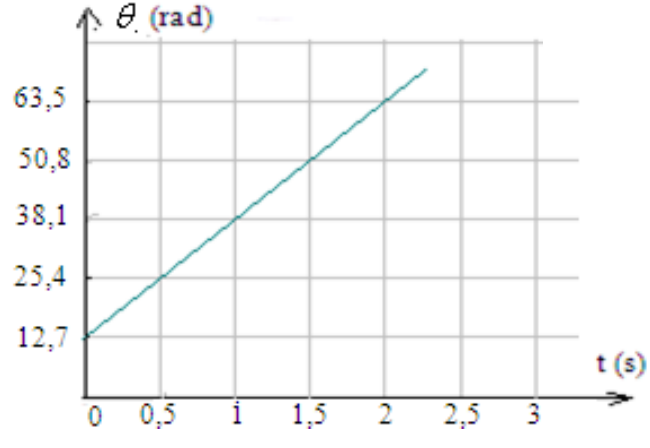
\includegraphics[width=0.4\textwidth]{./img/imgf00.png}
\end{enumerate}
 
%_________________partie 2  : gravitation universelle :)

\section*{Partie 2 : Le travail des forces agit sur un corps solide (8.5pts)}
\begin{wrapfigure}[5]{r}{0.3\textwidth}
  \begin{center}
    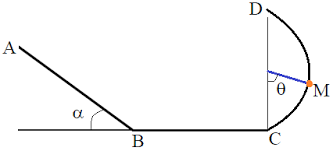
\includegraphics[width=0.3\textwidth]{./img/imgf01.png}
  \end{center}
\end{wrapfigure}


Un corps solide de masse m=2kg glisse sur un rail ABCD constitué de trois parties comme le montre la figure ci-dessous:
\\-Une partie AB incliné d’un angle $\alpha = 30^{\circ}$ par rapport à l’horizontale AB=1m.
\\-Une partie BC rectiligne BC=1m.
\\-Une partie CD circulaire de rayon r=40 cm.
\begin{enumerate}
    \item Calculer le travail du poids du corps durant le déplacement de A à B ?(1pt)
    \item \underline{sachant que la vitesse du corps de A  à B est constante} , déterminer le travail de la réaction du plan de contact puis en déduire la nature du contact ?\dotfill(2pt)
        \item Déterminer l’intensité f de la force de frottement durant le trajet AB?\dotfill(1pt)
        \item Calculer le travail du poids du corps durant le déplacement de B à C?\dotfill(1.5pt)
        \item Déterminer le travail du poids du corps durant le déplacement de C à M en fonction de m ,g , $\theta$ et r ?\dotfill(1pt)
        \item Quelle valeur doit prendre $\theta$ pour que : $W(\vec{P})_{A{\rightarrow}M} = 0 ?$\dotfill(2pts)
            \\On donne : g = 10N/Kg
\end{enumerate}
\end{document}
